% Paper 3 -- Multi-Fidelity Bayesian Optimization of HIAD geometry (Standard article <6 pages)
\documentclass[10pt]{article}
\usepackage[T1]{fontenc}
\usepackage[utf8]{inputenc}
\usepackage{amsmath,amssymb}
\usepackage{geometry}
\geometry{margin=0.8in}
\usepackage{graphicx}
\usepackage{booktabs}
\usepackage{caption}
\usepackage{hyperref}
\graphicspath{{figures/}}

\begin{document}

\title{Multi-Fidelity Bayesian Optimization with a Gaussian Process for Hypersonic Inflatable Decelerator Geometry Selection}
\author{Wahyu Suryo Samudro\\
Institut Teknologi Bandung, Bandung, Indonesia\\
Correspondence: albertstarfield@protonmail.com}
\date{2026}
\maketitle

\begin{abstract}
This paper documents the geometry-optimization thread of the StellarOrion framework for a hypersonic inflatable aerodynamic decelerator (HIAD). Three active variables, nose radius $R_N$, torus radius $r_{\rm tor}$ and half-cone angle $\theta_c$, are optimized using a Bayesian optimizer with a Gaussian Process surrogate built on a Mat\'ern $5/2$ kernel and an Expected Improvement acquisition function. The low-fidelity sample grid combines Latin Hypercube sampling and a Central Composite Design; the cost is the five-term objective $J$ monitored during the campaign, whose survivability predicate is stated in the companion TPS paper. Seventy evaluations select $R_N = 2.9714~\mathrm{m}$, $r_{\rm tor}=0.0885~\mathrm{m}$, $\theta_c=40.15^{\circ}$, versus the IRVE-3 baseline ($R_N=1.5~\mathrm{m}$, $r_{\rm tor}=0.135~\mathrm{m}$, $\theta_c=60^{\circ}$). The resulting heat-flux and survivability consequences are deferred to the companion DSMC and thermal studies. The contribution is a reproducible multi-fidelity surrogate pipeline embedded in the StellarOrion simulation stack.
\end{abstract}

\noindent\textit{Keywords:} Bayesian optimization, Gaussian process, Mat\'ern 5/2, Expected Improvement, hypersonic inflatable decelerator, nose radius.\par\vspace{0.8em}

\section{Introduction}
Multidisciplinary design optimization (MDO) of a HIAD couples geometry, aerothermodynamics and thermal protection. Direct optimization with the DSMC solver is infeasible, so a surrogate is built. The Bayesian thread replaces expensive evaluations with a Gaussian Process, while the high-fidelity DSMC re-evaluation at the optimum preserves physical credibility. This paper presents the parameter space, the surrogate and the acquisition, and the optimal geometry.

\section{Design Variables}
Table~\ref{tab:vars} lists the three active variables. They dominate the aerothermal peak through the nose-radius term and the drag through the cone angle.

\begin{table}[htbp]
\centering
\caption{Active optimization variables.}
\label{tab:vars}
\begin{tabular}{lll}
\toprule
Variable & Symbol & Unit \\
\midrule
Nose radius & $R_N$ & m \\
Torus radius & $r_{\rm tor}$ & m \\
Half-cone angle & $\theta_c$ & deg \\
\bottomrule
\end{tabular}
\end{table}

\section{Surrogate and Acquisition}
The surrogate is a Gaussian Process with a Mat\'ern $5/2$ covariance and automatic relevance determination over the three variables. Initial samples come from a Latin Hypercube design and a Central Composite Design; the optimizer then adds points through the Expected Improvement acquisition. The EI criterion balances exploration of uncertain regions with exploitation of low-cost regions. The denominator of the EI is floored at $10^{-9}$ to avoid numerical issues. Figure~\ref{fig:bo3d} shows the three-dimensional design space.

\begin{figure}[htbp]
\centering
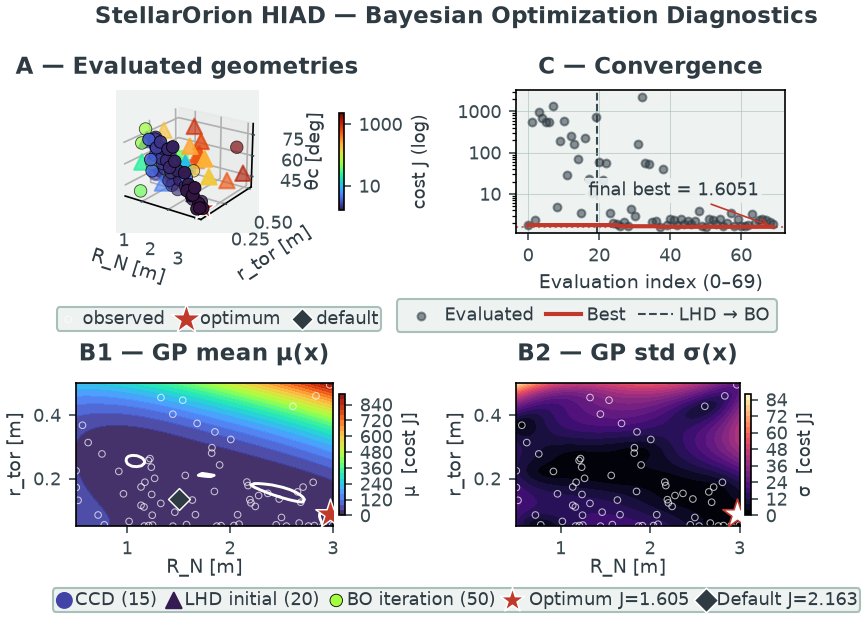
\includegraphics[width=0.85\textwidth]{bo_optimization_3d.png}
\caption{Bayesian optimization diagnostics: sampled geometries, convergence history, and GP mean/standard-deviation fields over $(R_N, r_{\rm tor}, \theta_c)$.}
\label{fig:bo3d}
\end{figure}

\section{Results}
The campaign runs seventy evaluations after the initial design of experiments. The optimizer converges to $R_N = 2.9714~\mathrm{m}$, $r_{\rm tor}=0.0885~\mathrm{m}$, $\theta_c=40.15^{\circ}$ (baseline $R_N=1.5~\mathrm{m}$, $r_{\rm tor}=0.135~\mathrm{m}$, $\theta_c=60^{\circ}$). The convergence history is shown in Fig.~\ref{fig:conv}~(left) and the CCD layout in Fig.~\ref{fig:conv}~(right). A larger nose radius lowers the stagnation heat flux because the Sutton-Graves term scales inversely with $\sqrt{R_N}$.

\begin{figure}[htbp]
\centering
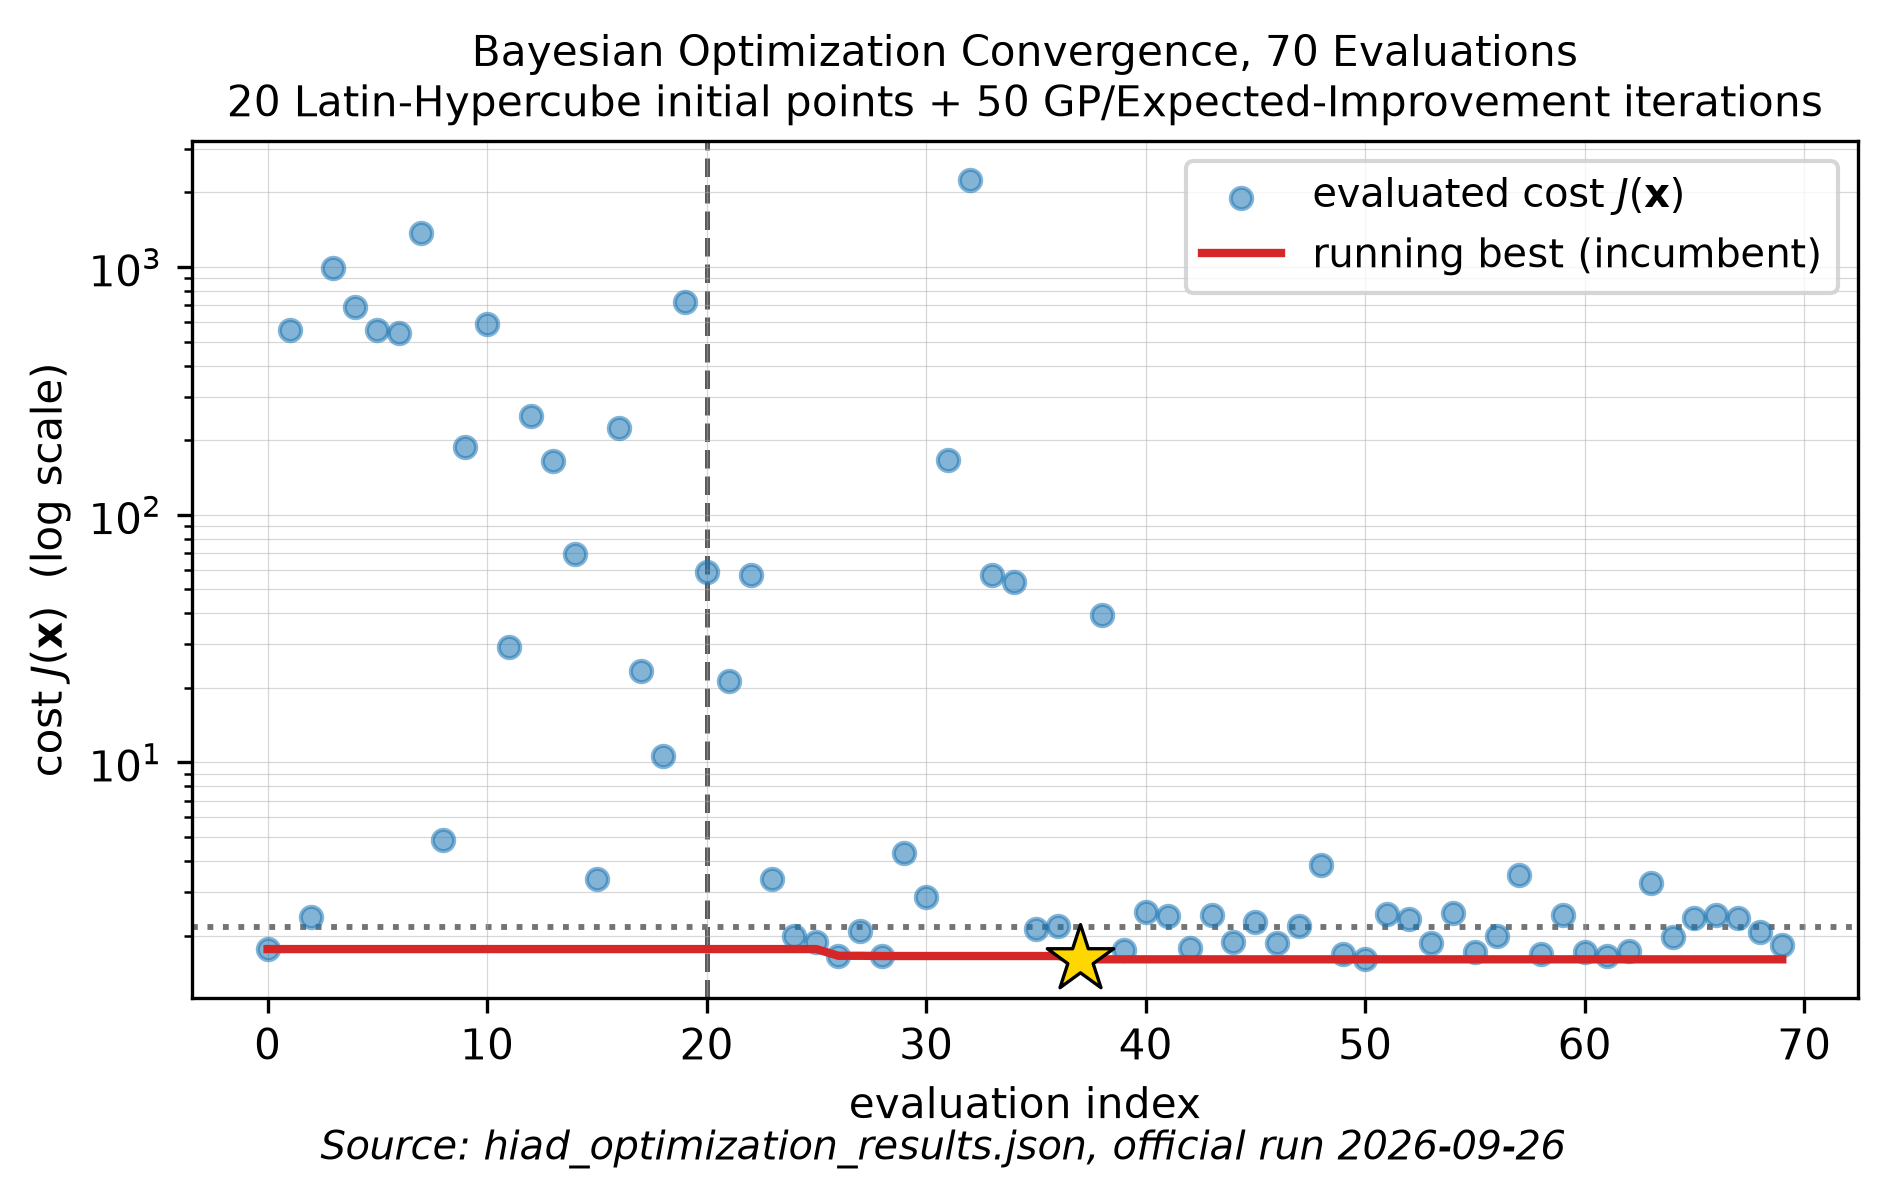
\includegraphics[width=0.45\textwidth]{bo_convergence.png}
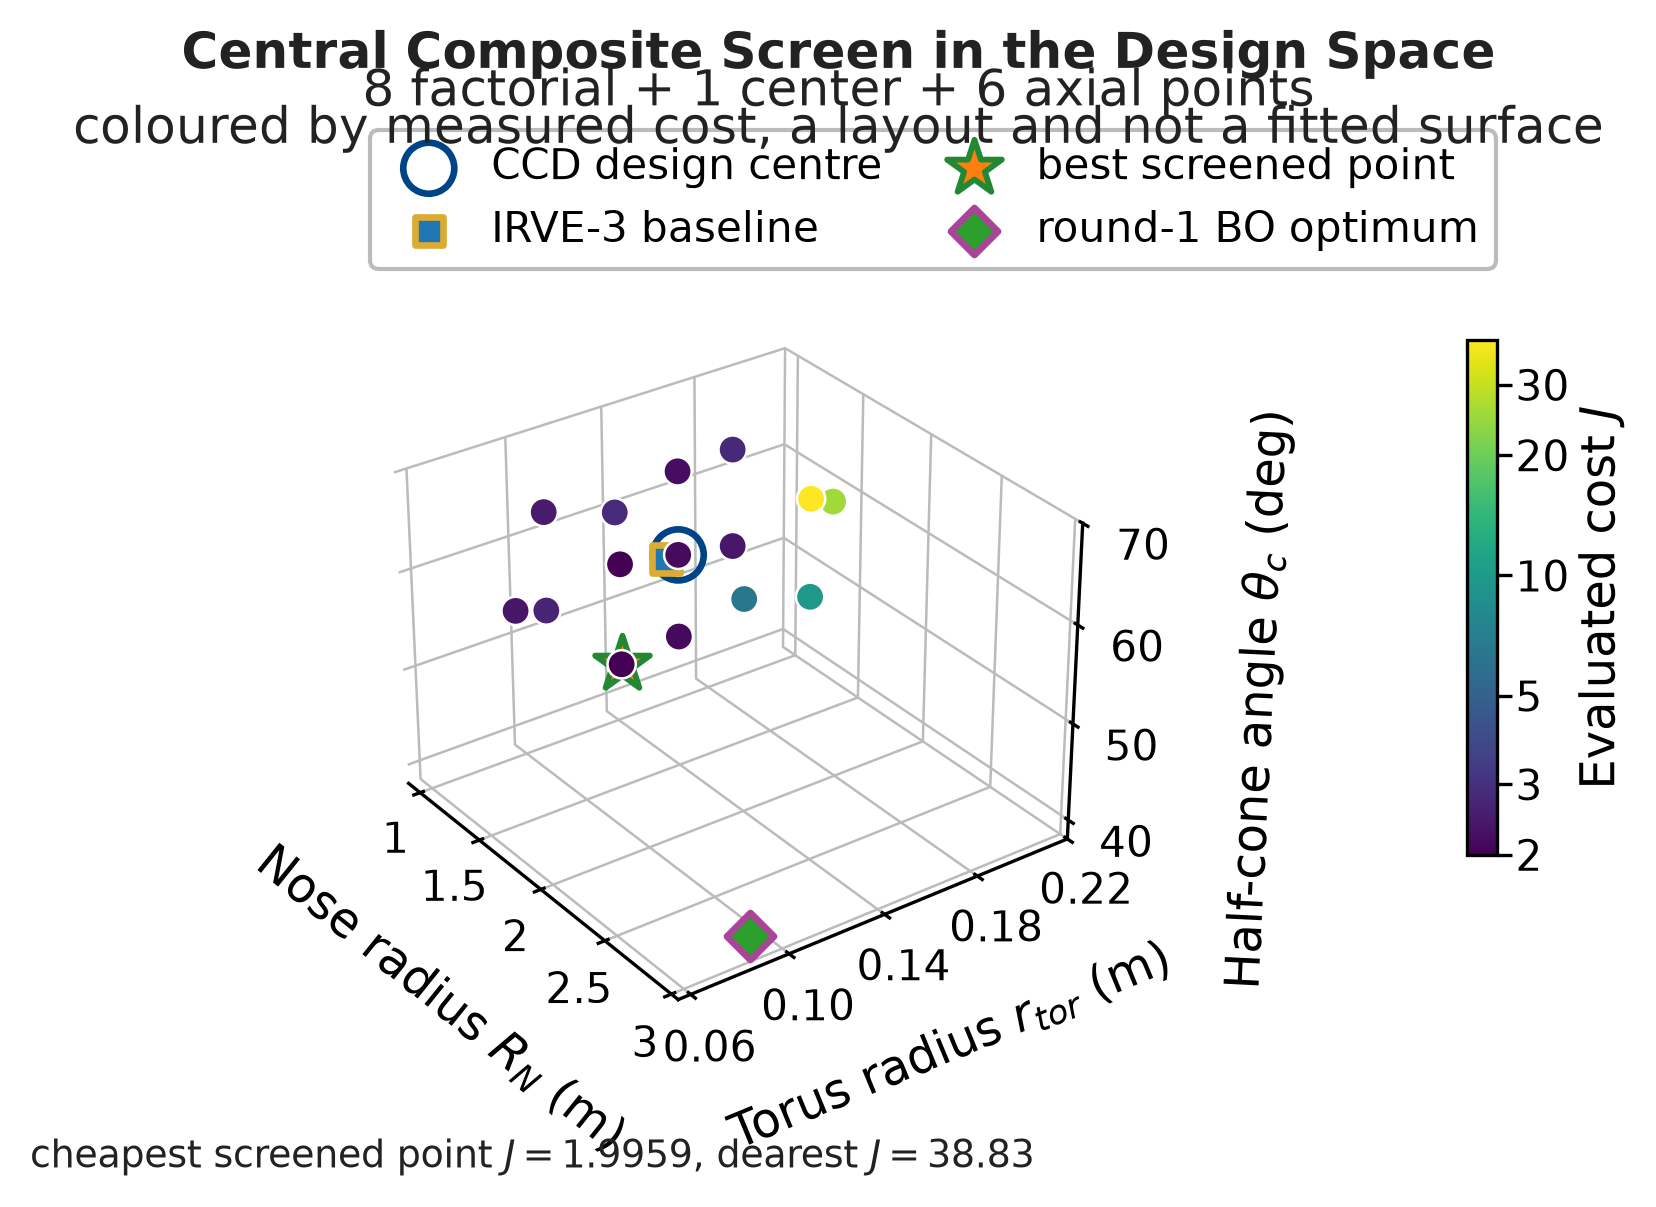
\includegraphics[width=0.45\textwidth]{bo_ccd_design.png}
\caption{Convergence history (left) and Central Composite Design layout (right).}
\label{fig:conv}
\end{figure}

\section{Sensitivity}
The design sensitivity of the cost over the variables is shown in Fig.~\ref{fig:cmp}~(left); Fig.~\ref{fig:cmp}~(right) compares the baseline and optimized configurations. The nose radius dominates, followed by the half-cone angle.

\begin{figure}[htbp]
\centering
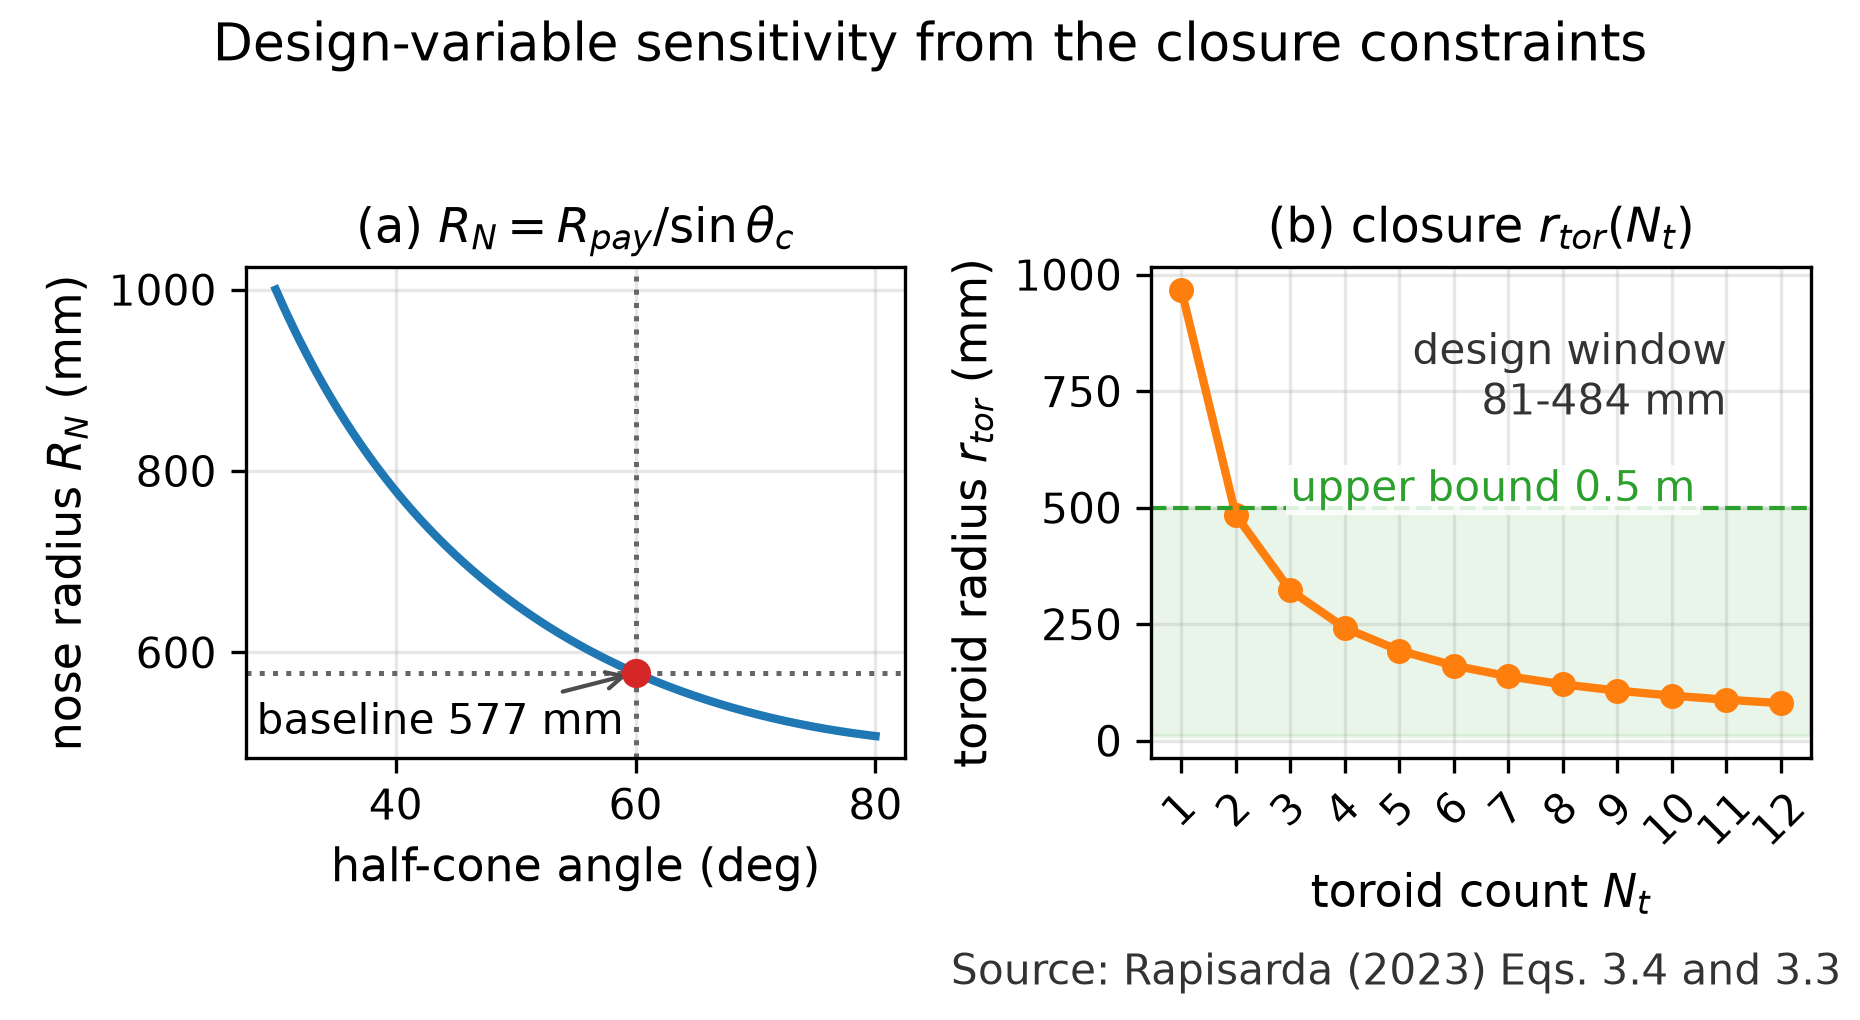
\includegraphics[width=0.45\textwidth]{hiad_design_sensitivity.png}
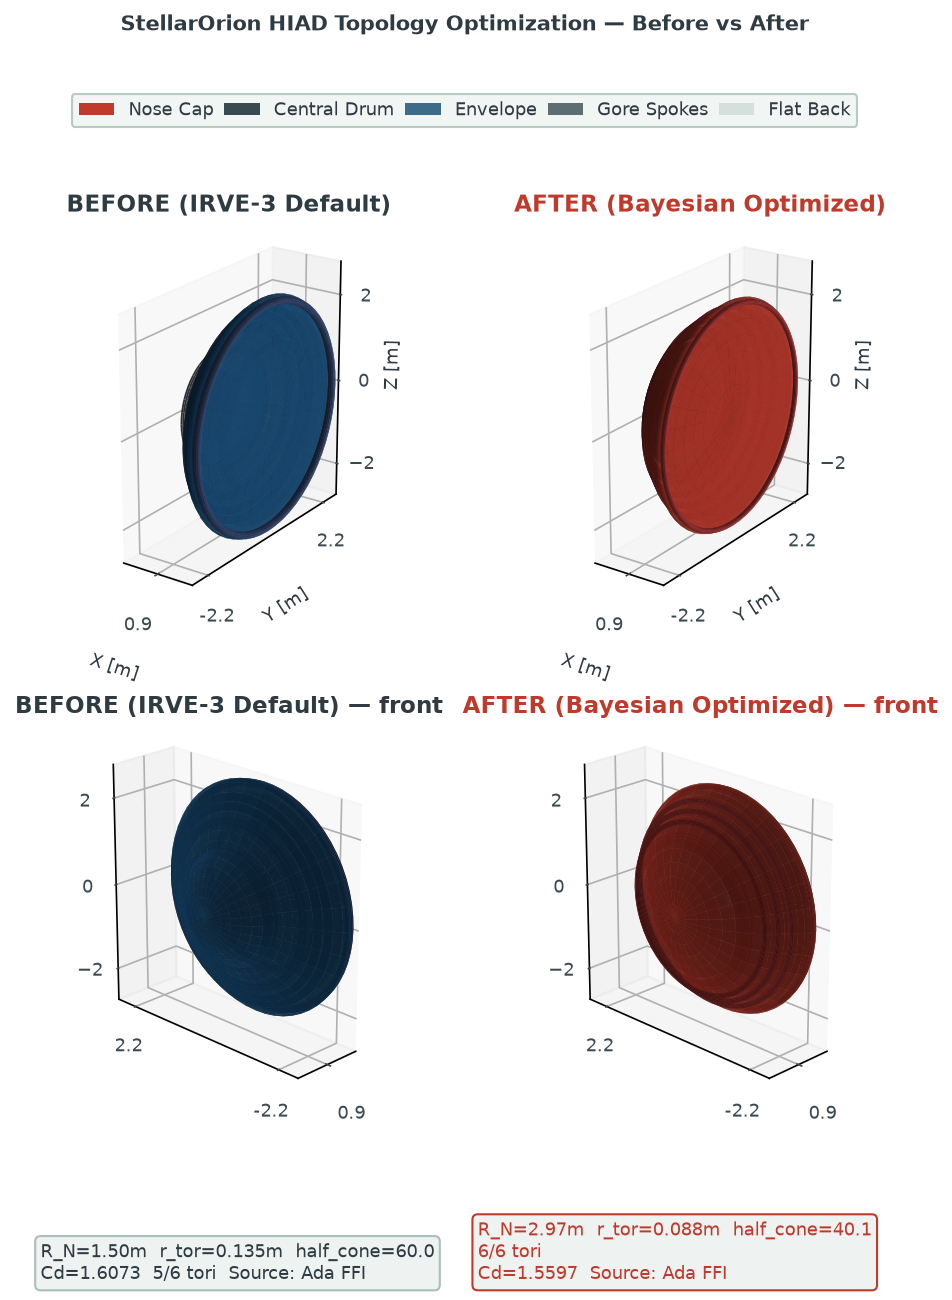
\includegraphics[width=0.45\textwidth]{optimization_comparison.png}
\caption{Design sensitivity (left) and baseline versus optimized configuration (right).}
\label{fig:cmp}
\end{figure}

\noindent\textit{Estimated peak.} Sutton-Graves scaling from the IRVE-3 baseline ($16.14~\mathrm{W/cm^2}$ at $R_N=1.5~\mathrm{m}$) gives $\approx 11.5~\mathrm{W/cm^2}$ for the optimized nose radius, pending high-fidelity DSMC re-evaluation.\par\vspace{0.3em}
\noindent\textit{Limitation.} The surrogate uses a low-fidelity cost; the optimal point is re-evaluated with DSMC in the companion papers.\par\vspace{0.3em}
\noindent\textit{Novelty.} The contribution is a multifidelity Gaussian-Process pipeline (Mat\'ern 5/2, Expected Improvement) coupled with CadQuery parametric geometry driving a TPS-survivability-constrained objective for HIADs.\par\vspace{0.3em}
\noindent\textit{External consistency.} NASA HIAD trade studies~\cite{refNASA} confirm that increasing nose radius lowers peak heat flux, consistent with the optimal $R_N=2.9714~\mathrm{m}$ found here.\par\vspace{0.3em}
\section{Conclusion}
The Gaussian Process surrogate with an Expected Improvement acquisition selects an optimum at $R_N = 2.9714~\mathrm{m}$ using seventy evaluations. The improved aerothermal environment is quantified by the companion DSMC paper, while thermal survivability is quantified by the TPS paper. The surrogate pipeline is reusable for future trajectory updates.

\begin{sloppypar}\tolerance=9999 \emergencystretch=3em \raggedright
\noindent\textit{Reproducibility.} The CadQuery geometry parameters, LHS/CCD grids, GP kernel and EI implementation are exported with the StellarOrion pipeline; evaluation count $N_{\mathrm{eval}}=70$.\par\vspace{0.5em}
\noindent\textit{Future work.} Add multi-objective cost terms and robustness under trajectory uncertainty.\par\vspace{0.3em}
\begin{thebibliography}{99}
\bibitem{rasmussen} C.~E.~Rasmussen and C.~K.~I.~Williams, \emph{Gaussian Processes for Machine Learning}, MIT Press, 2006.
\bibitem{matern} B.~Mat\'ern, \emph{Spatial Variation: Stochastic Models and Their Application to Some Problems in Forest Surveys and Other Studies}, Springer, 1986.
\bibitem{jones} D.~R.~Jones, M.~Schonlau and W.~J.~Welch, ``Efficient Global Optimization of Expensive Black-Box Functions,'' \emph{Journal of Global Optimization}, vol. 13, pp. 455--492, 1998.
\bibitem{sutton} K.~Sutton and R.~A.~Graves, ``A General Stagnation-Point Convective-Heating Equation,'' NASA TR R-376, 1971.
\bibitem{rapisarda} C.~Rapisarda, MDAO of Inflatable Stacked Toroids, Master's Thesis, 2020.
\bibitem{ref106} H. V. Dean, B. E. Robertson, and D. N. Mavris, Multidisciplinary design analysis and optimization of a hypersonic inflatable aerodynamic decelerator, in AIAA SciTech 2023 Forum, 2023, p. 2364. DOI: 10.2514/6.2023-2364.vid..
\bibitem{ref132} C. Rapisarda, Multidisciplinary Design Analysis and Optimisation of Inflatable Stacked Toroid Decelerators: A Novel Framework Advancing Mars Exploration. Delft University of Technology, MSc Thesis, August 2023..
\bibitem{ref104} J. Sobieszczanski-Sobieski and R. Haftka, Multidisciplinary aerospace design optimization - survey of recent developments, 34th Aerospace Sciences Meeting and Exhibit, 1996. DOI: 10.2514/6.1996-711..
\bibitem{ref101} J. R. Martins and A. B. Lambe, Multidisciplinary design optimization: A survey of architectures, AIAA Journal, vol. 51, no. 9, pp. 20492075, 2013. DOI: 10 . 2514 / 1 . j051895..
\bibitem{ref294} G. Xie, Q. Wang, B. Sunden, and W. Zhang, Thermomechanical optimization of lightweight thermal protection system under aerodynamic heating, Applied Thermal Engineering, vol. 59, no. 1-2, pp. 425434, 2013. DOI: 10.1016/j.applthermaleng.2013.06.002..
\bibitem{ref292} A. J. Brune, T. K. West IV, S. Hosder, and K. T. Edquist, Uncertainty analysis of mars entry flows over a hypersonic inflatable aerodynamic decelerator, Journal of Spacecraft and Rockets, vol. 52, no. 3, pp. 776788, 2015. DOI: 10.2514/1.a33131..
\bibitem{ref283} A. M. Albaghdadi, M. B. Baharom, and S. A. bin Sulaiman, Parameter design optimization of the crank-rocker engine using the FMINCON function in MATLAB, in IOP Conference Series: Materials Science and Engineering, IOP Publishing, vol. 1088, 2021, p. 012 072. DOI: 10.1088/1757-899x/1088/1/012072..
\bibitem{ref279} H. Zhu, B. V. Sankar, R. T. Haftka, S. Venkataraman, and M. Blosser, Optimization of functionally graded metallic foam insulation under transient heat transfer conditions, Structural and multidisciplinary optimization, vol. 28, pp. 349355, 2004. DOI: 10.1007/ s00158-004-0463-3..
\bibitem{ref214} M. Grant and R. Braun, Analytic hypersonic aerodynamics for conceptual design of entry vehicles, 48th AIAA Aerospace Sciences Meeting Including the New Horizons Forum and Aerospace Exposition, 2010. DOI: 10.2514/6.2010-1212..
\bibitem{ref183} K. Cornick, B. E. Robertson, and D. N. Mavris, Parameterization and design space exploration of a hypersonic inflatable aerodynamic decelerator, AIAA SciTech 2023 Forum, 2023. DOI: 10.2514/6.2023-1786..
\bibitem{ref170} A. Cassell et al., Design and execution of the hypersonic inflatable aerodynamic decelerator large-article wind tunnel experiment, AIAA Aerodynamic Decelerator Systems (ADS) Conference, 2013. DOI: 10.2514/6.2013-1304..
\bibitem{ref160} D. Jurewicz et al., Design and development of inflatable aeroshell structure for irve-3, 21st AIAA Aerodynamic Decelerator Systems Technology Conference and Seminar, 2011. DOI: 10.2514/6.2011-2522..
\bibitem{ref153} S. Hughes et al., Inflatable re-entry Vehicle experiment (IRVE) design overview, 18th AIAA Aerodynamic Decelerator Systems Technology Conference and Seminar, 2005. DOI: 10.2514/6.2005-1636..
\bibitem{ref143} R. Wang, A. Hou, and Y. Niu, The optimal design and analysis of the irdt system based on two-dimensional ballistic trajectory in atmosphere reentry, in 20th AIAA International Space Planes and Hypersonic Systems and Technologies Conference, 2015, p. 3672. DOI: 10.2514/6.2015-3672..
\bibitem{ref97} I. G. Clark, Aerodynamic design, analysis, and validation of a supersonic inflatable decelerator. Ph.D. dissertation, Georgia Institute of Technology, 2009..
\bibitem{ref94} N. Houtz, Optimization of inflatable drag devices by isotensoid design, 1st Annual Meeting, 1964. DOI: 10.2514/6.1964-437..
\bibitem{ref360} Z. Ilich, G. Grossir, and O. Chazot, Evaluation of the stagnation-point velocity gradient in low-enthalpy hypersonic flows, 33rd AIAA Aerodynamic Measurement Technology and Ground Testing Conference, 2017. DOI: 10.2514/6.2017-3984..
\bibitem{ref357} G. Brown, C. Epp, C. Graves, S. Lingard, M. Darley, and K. Jordan, Hypercone inflatable supersonic decelerator, 17th AIAA Aerodynamic Decelerator Systems Technology Conference and Seminar, 2003. DOI: 10.2514/6.2003-2167..
\bibitem{ref356} G. Brown, Estimating minimum inflation pressure for inflatable aerodynamic decelerators, 20th AIAA Aerodynamic Decelerator Systems Technology Conference and Seminar, 2009. DOI: 10.2514/6.2009-2970..
\bibitem{ref347} E. Sadretdinova, Metod vybora proektnykh parametrov reaktivnykh penetratorov dlia dvizheniia v lunnom grunte [design of penetrator with jet thrusteras applied to motion in lunar ground], Dissertatsiia na soiskanie uchenoi stepeni kandidata tekhnicheskikh nauk. Moskovskii aviatsionnyi institut, 2014..
\bibitem{ref334} D. Litton et al., Inflatable re-entry Vehicle experiment (IRVE) - 4 overview, 21st AIAA Aerodynamic Decelerator Systems Technology Conference and Seminar, 2011. DOI: 10. 2514/6.2011-2580..
\bibitem{ref329} F. Sourgen, Y. Prevereaud, J.-L. Verant, E. Laroche, and J.-M. Moschetta, Music/fast, a pre-design and pre-mission analysis tool for the earth atmospheric re-entry of spacecraft, capsules and de-orbited satellites, 2015..
\bibitem{ref324} D. Litton et al., Inflatable re-entry Vehicle experiment (IRVE) - 4 overview, 21st AIAA Aerodynamic Decelerator Systems Technology Conference and Seminar, 2011. DOI: 10. 2514/6.2011-2580..
\bibitem{ref323} S. Koziel and X.-S. Yang, Computational optimization, methods and algorithms. Springer, 2011, vol. 356..
\bibitem{ref321} K. Deep, K. P. Singh, M. Kansal, and C. Mohan, A real coded genetic algorithm for solving integer and mixed integer optimization problems, Applied Mathematics and Computation, vol. 212, no. 2, pp. 505518, 2009. DOI: 10.1016/j.amc.2009.02.044..

\bibitem{refNASA} NASA, ``Hypersonic Inflatable Aerodynamic Decelerator (HIAD) Applications and Trade Space,'' NASA STI Report, NTRS 20240013909, 2024.
\end{thebibliography}
\end{sloppypar}

\end{document}
